\documentclass[a4paper,11pt]{article} 

\usepackage[T1]{fontenc}
\usepackage[utf8]{inputenc}

\usepackage{multirow} 
\usepackage{booktabs} 
\usepackage{graphicx} 
\usepackage{setspace}
\usepackage[skip=6pt plus1pt, indent=0pt]{parskip}

\usepackage{float}
\usepackage{fancyhdr}

\usepackage{tcolorbox}
\usepackage{hyperref}
\hypersetup{
    colorlinks=true,
    linkcolor=blue,
    filecolor=magenta,      
    urlcolor=blue
}
\usepackage{minted}
\usepackage[margin=1in]{geometry}
\usepackage{caption}

\newcommand{\incode}[1]{
\begin{tcolorbox}[colback=blue!5!white, boxrule=0mm, sharp corners]
\texttt{#1}
\end{tcolorbox}
}

\newcommand{\note}[1]{\textit{\textcolor{gray}{#1}}}

\pagestyle{fancy} 
\fancyhf{} 
\lhead{Advanced Computer Networks 2022}
\rhead{Lin Wang, George Karlos, Florian Gerlinghoff} 
\cfoot{\thepage} 

\begin{document}


\thispagestyle{empty} 

\begin{tabular}{@{}p{15.5cm}} 
{\bf Advanced Computer Networks 2022} \\
Vrije Universiteit Amsterdam  \\ Lin Wang, George Karlos, Florian Gerlinghoff\\
\hline 

\end{tabular} 

\vspace*{0.3cm} 

{\LARGE \bf Lab3: Building Your Data Center Network (Report)} 

\vspace*{0.3cm} 

%============== Please do not change anything above ==============%

% Please modify this part with your group information
\begin{tcolorbox}[sharp corners, colback=blue!5!white]
\begin{tabular}{@{}ll}
\textbf{Group number:} & 9 \\
\textbf{Group members:} & Hsiang-ling Tai, Yung-sheng Tu, Sicheng Peng \\
\textbf{Slip days used:} & 0 \\
\end{tabular}
\end{tcolorbox}

\vspace{0.4cm}

% Please do not remove any of the section headings below

\section{Building a Fat-Tree Data Center Network in Mininet}
\begin{itemize}
    \item Enumerate all the switches from ft\_topo and call addSwitch() function to add each switch.
    \item Enumerate all the host from ft\_topo and call addHost() function to add each host and also set up the IP address based on Fat-tree paper.
    \item Enumerate all the edges in all the switches (would ignore the edge if already add the link between the nodes) and call addLink to setup a bandwidth 15Mbps and delay 5ms on every links.
\end{itemize}


\section{Implementing Shortest-Path Routing in the Fat-Tree Network}
\subsection{Topology Discovery}
\begin{itemize}
    \item Use get\_switch() function to discover all switches and map \textit{Datapath ID} to \textit{fat-tree Node} instance.
\end{itemize}
\subsection{Setting up Dijkstra's Algorithm}
\begin{itemize}
    \item Initialisation \\
    Calculate all the shortest paths and store them in my Dijkstra object.
    \item Get the Shortest Path \\
    Simply call its get\_path() function to get the shortest path between two edge switches.
\end{itemize}
\subsection{ARP Resolution with Dijkstra's Algorithm}
\begin{itemize}
    \item ARP Request \\
    When switches receive an ARP request, it would have \textit{in\_port} and \textit{source's IP address} information.
    \begin{itemize}
        \item Add flow \\
        Add the flow entry whose Match is the source's IP address and whose Action is outputting the packet to \textit{in\_port}.
        \item Add mapping to ip\_to\_port \\
        Bind the host's IP and the port of the current switch.
        \item Add mapping to ip\_to\_dpid \\
        Bind the host's IP and the Datapath ID of the first switch the packet arrived.\\
    \end{itemize}
    \item Flooding with Dijkstra's Algorithm
    \begin{itemize}
        \item Find the Shortest Paths to Other Edge Switches
        \begin{itemize}
            \item Finding the First Switch of this Packet \\
            Get the node (first switch) mentioned in section 2.1 by using the Datapath ID mentioned in section 2.3 as a key.
            \item Finding the Next Nodes where the Packet should be Sent \\
            Use the Datapath Id of the current switch to find out where it is in all paths and get the next node in all paths.
            \item Finding the Ports of All Next Nodes \\
            Get all links of this switch with get\_link() function and find the ports corresponding to all next nodes.
        \end{itemize}
        \item Flooding \\
        In this case, since the flooding path is the shortest, it would not cause loops and also the ARP packets will be sent with the shortest paths.
    \end{itemize}
    \item ARP Response \\
    There is a ip\_to\_port mapping set up during ARP requests in the controller. The packet of ARP Response would always be forwarded to the controller and then the controller would look up the mapping and forward it to the corresponding port.
\end{itemize}
\subsection{IPv4 Packet Forwarding}
Since the flow entries added on each switch are all the rules of the shortest paths while ARP broadcast, the switch getting the packet would not ask the controller again and forward packets with the shortest paths.

\section{Implementing Two-Level Routing in the Fat-Tree Network}
\subsection{Topology Discovery}
\begin{itemize}
    \item Use get\_switch() function to discover all switches and map \textit{DatapathID} to Fat-tree Node instance.
    \item Use get\_link() function to discover all links and map a port to IP address for every switch. For example, the switch with \textit{DatapathID 11} has 4 ports and the link on \textit{port 3} is connected to the Node with IP address \textit{'10.0.0.1'}.
    \begin{minted}{python}
    {
        11: {3: '10.0.0.1', 2: '10.4.1.2', 1: '10.4.1.1', 4: '10.0.1.1'}, 
        12: {4: '10.1.1.1', 3: '10.1.0.1', 1: '10.4.2.1', 2: '10.4.2.2'}
    }
    \end{minted}
    
\end{itemize}

\subsection{Setting up Two-Level Routing Table}
We set up the two-level routing rule and add the flow entry based on which kind of switch it is.
\begin{itemize}
    \item Core Switch\\
    As mentioned in \textit{section 3.1}, we have already set up a mapping from port to IP address.  So, the Match would be the Prefix <IP address>/16, and the Action would be Outputting the packet to the port which map with the IP address.
    \item Aggregation Switch\\
    Ports can be classified into upper ports and lower ports in every aggregation switch.  And the priority of the lower port's flow entries is higher than the upper port's flow entries.  Otherwise, all the packets would match the upper port's rule and be forwarded outside the pod.
    \begin{itemize}
        \item Lower Port\\
        Connected with edge switches. Its Match would be Prefix <IP address>/24, and the Action would be outputting the packet to the mapped port.
        \item Upper Port\\
        Connected with core switch.  Its Match would be Suffix <IP address>/8, and the Action would also be outputting the packet to the mapped port.
    \end{itemize}
    \item Edge Switch\\
    Ports can also be classified into upper ports and lower ports in every aggregation switch.  However, the get\_link() function cannot obtain the links between hosts and switches, so the lower port's flow entries are set up during ARP Resolution (see section 3.3).  Again, the priority of the lower port's entries is higher than the upper port's.
    \begin{itemize}
        \item Lower Port\\
        Connected with edge switches. Its Match would be Prefix <IP address>/32, and the Action would be outputting the packet to the mapped port. (see ARP Request in section 3.3)
        \item Upper Port\\
        Connected with aggregation switch.  Its Match would be Suffix <IP address>/8, and the Action would be outputting the packet to the mapped port.
    \end{itemize}
\end{itemize}
\subsection{ARP Resolution}
\begin{itemize}
    \item ARP Request\\
    When edge switches receive an ARP request, it would have \textit{in\_port} and \textit{source's IP Address} information.  So, we can add the flow entry whose Match is the source's IP address and Action is outputting the packet to \textit{in\_port}.
    \item Flooding\\
    In this case, we cannot simply flood to all ports except in port because it would cause loops.  So we divide into 2 flooding strategies.
    \begin{itemize}
        \item Flood to all lower ports\\
        If core switch receives an ARP request, flood to all lower ports except in\_port.  If the aggregation switch or edge switch receives an ARP request from the upper port, flood to all lower ports.
        \item Flood to all lower ports and one upper port\\
        If the aggregation switch or edge switch receives ARP requests from the lower port, flood to all lower ports except in\_port.  For the edge switch, forwarding ARP requests to only one upper port can prevent loops. For the aggregation switch, forwarding ARP requests to only one upper port can reduce the ARP request packet.
    \end{itemize}
    \item ARP Reply\\
    There is a mac\_to\_port mapping set up during ARP requests in the controller.  The ARP Reply packet would always be forwarded to the controller, and then the controller would look up the mapping and forward it to the corresponding port.
\end{itemize}


\section{Comparing the Performance of the Two Routing Schemes}

\subsection{Experiment 1 — Multiplexing Congestion}
\begin{itemize}
    \item Motivation \\
    In the shortest path method, the overlapped proportion of all paths is much higher than the counterpart of two-level routing. The two-level routing algorithm would forward packet to different port based on the hostID, which equally share the resource of the whole internet. So, when multiple streams are on the internet at the same time, the shortest path routing is expected to occur more congestion compared with the two-level.
    \item Methodology
    \begin{enumerate}
        \item Stream on 2 pairs of host \\
        We send packet \textbf{from 10.1.0.2 to 10.0.0.2} and \textbf{from 10.1.0.3 to 10.0.0.3}.  In shortest path routing, both streams would pick same edge switch, same aggregation switch, and core switch to forward the packet.  In contrast, two-level routing would pick different aggregation switch and core switch.  So, shortest path routing should lead to congestion.
        \begin{figure}[htbp]
        \centering
        \centering
        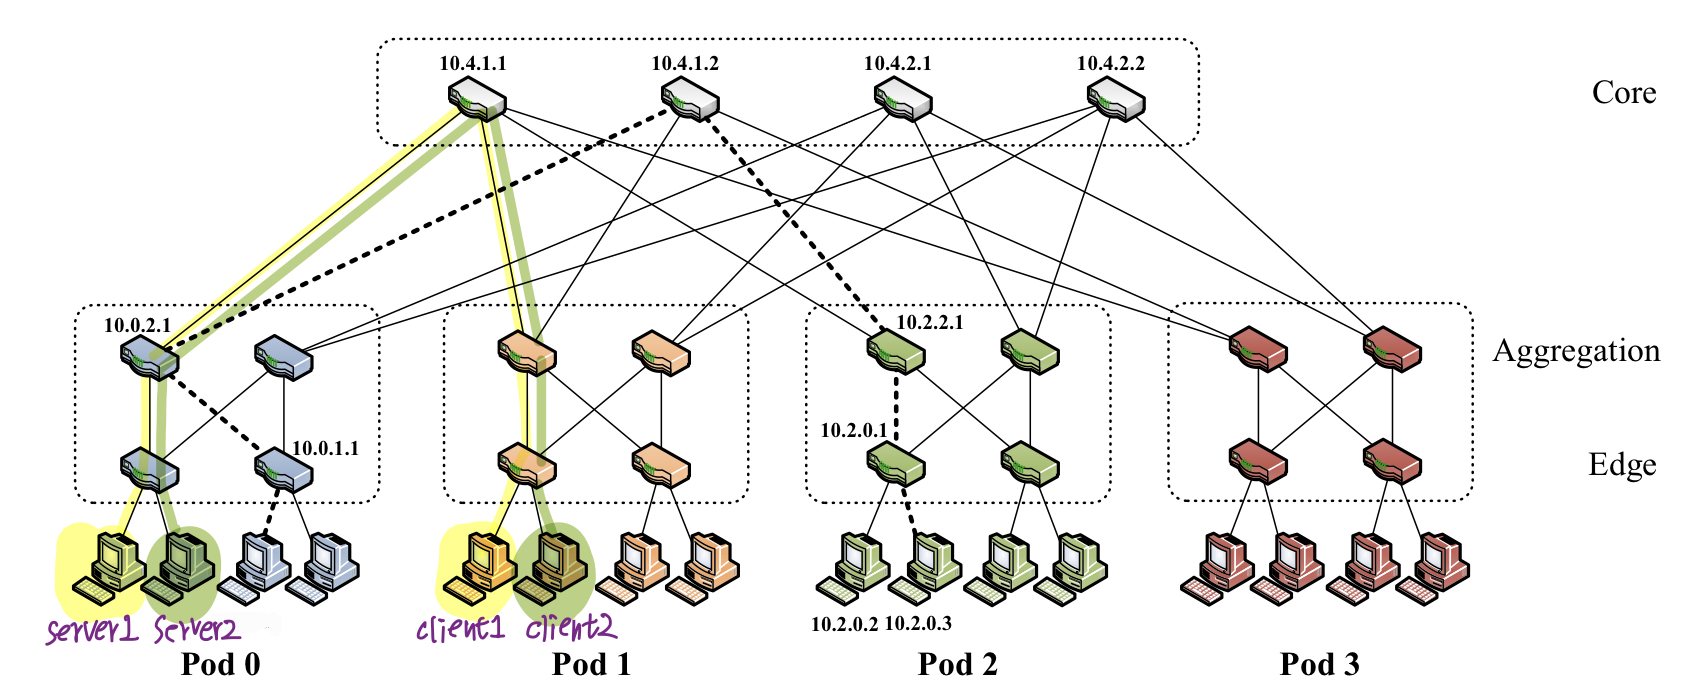
\includegraphics[width=14cm]{sprouting.jpeg}
        \caption{The path is overlapped using the shortest path routing}
        \label{fig:sp}
        \end{figure}
        \begin{figure}[htbp]
        \centering
        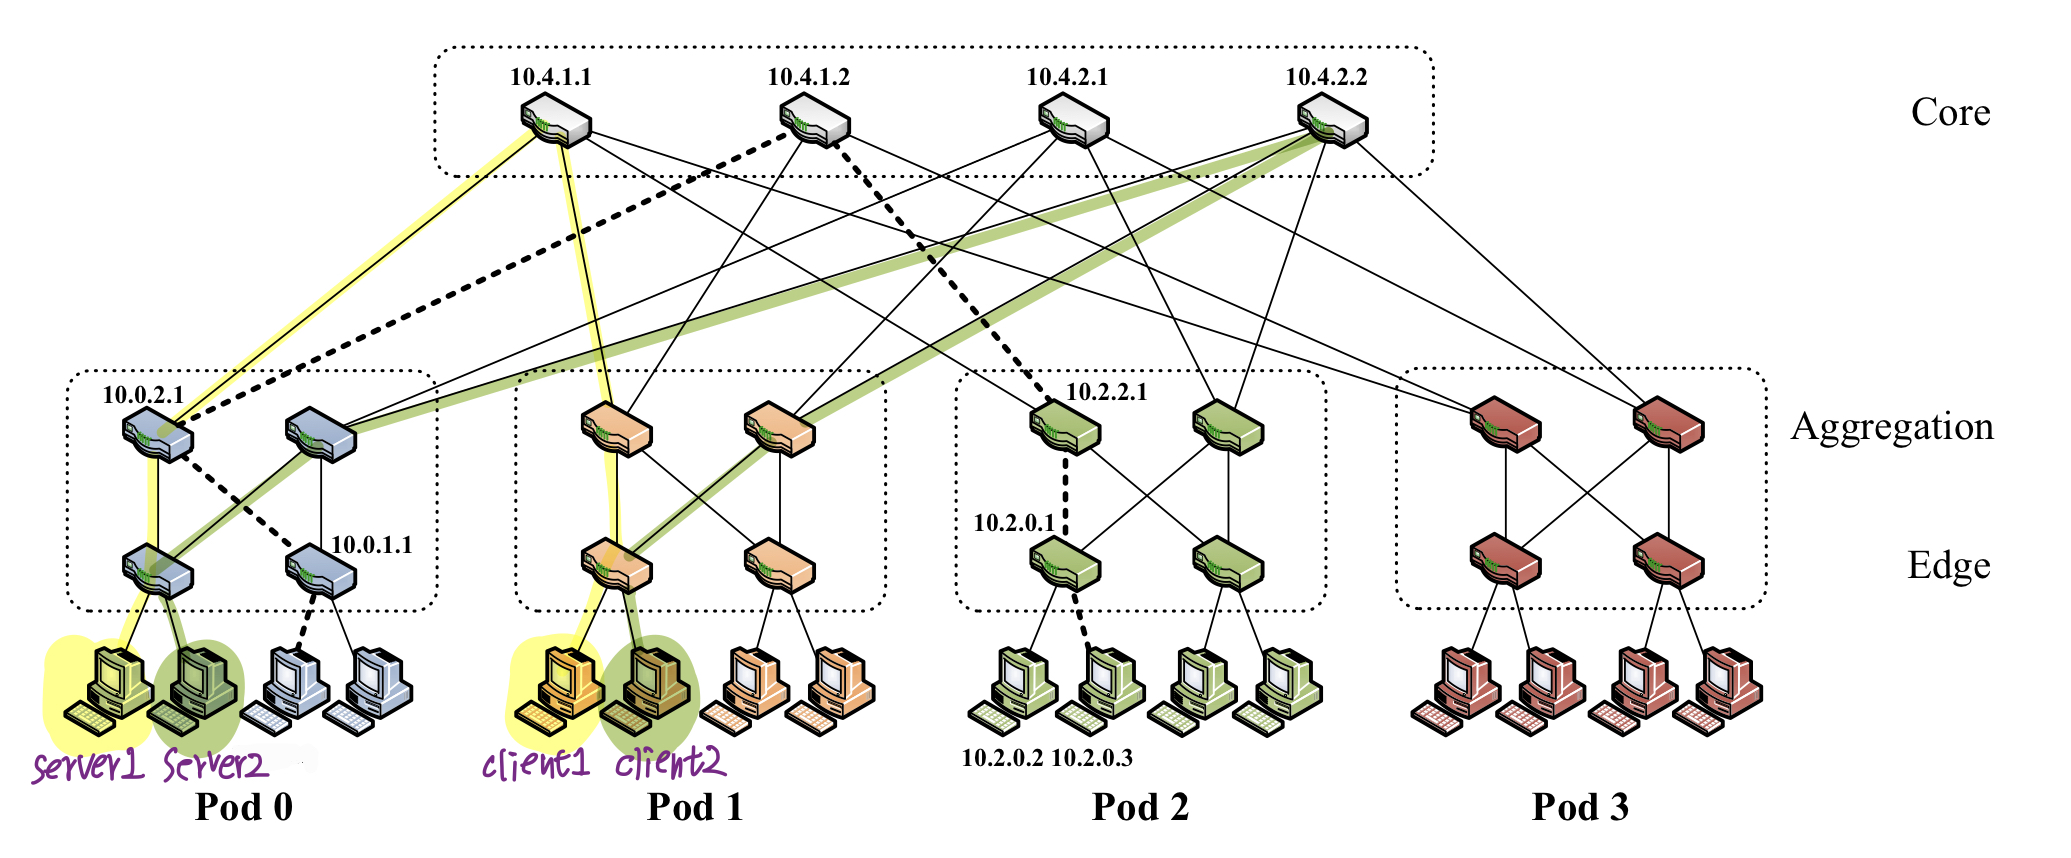
\includegraphics[width=14cm]{ftrouting.jpeg}
        \caption{Two-level routing chooses different switches to route based on destination host ID}
        \label{fig:ft}
        \end{figure}
        \item Experiment Data \\
        To guarantee the result would not impact by extrema.  We use iperf3 and set parameter\textbf{ -t 20} on client side, which would send packets to server over 20 seconds.
    \end{enumerate}
    \item Results \\
    Figure \ref{fig:e1sp} and Figure \ref{fig:e2sp} show that sending packets with the shortest path routing would lead to \textbf{547 retries on client 10.1.0.2} and \textbf{2141 retries on client 10.1.0.3}.  In contrast, Figure 3 and Figure 4 show that two-level routing would only have \textbf{7 retries on client 10.1.0.2} and \textbf{66 retries on client 10.1.0.3}.
    \captionsetup{width=7cm}
    \begin{figure}[htbp]
    \centering
    \begin{minipage}[t]{0.49\textwidth}
    \centering
    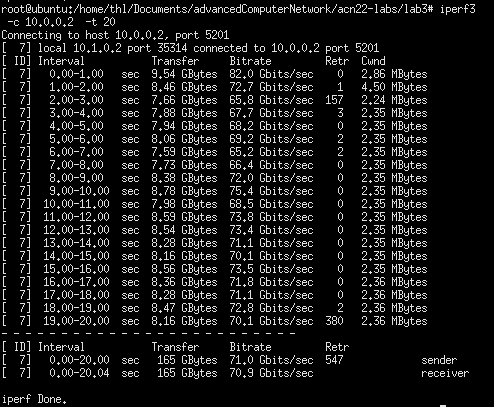
\includegraphics[width=7.5cm]{h002-h102-sp.png}
    \caption{Send packets from 10.1.0.2 to 10.0.0.2 with the shortest path}
    \label{fig:e1sp}
    \end{minipage}
    \begin{minipage}[t]{0.49\textwidth}
    \centering
    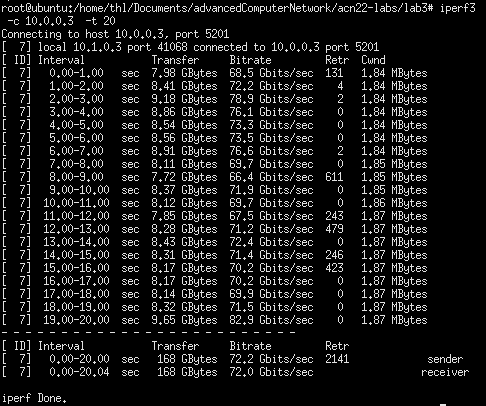
\includegraphics[width=7.5cm]{h003-h103-sp.png}
    \caption{Send packets from 10.1.0.3 to 10.0.0.3 with the shortest path}
    \label{fig:e2sp}
    \end{minipage}
    \end{figure}
    \begin{figure}[htbp]
    \centering
    \begin{minipage}[t]{0.49\textwidth}
    \centering
    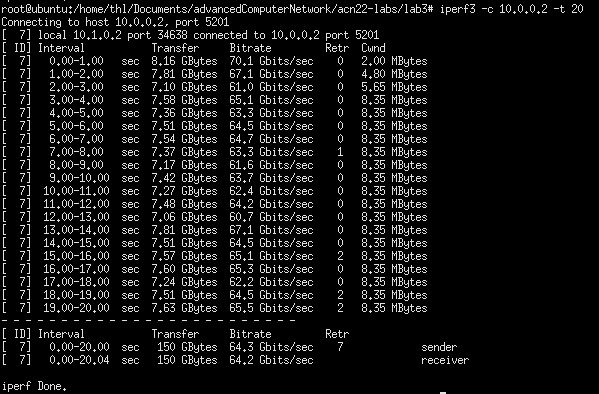
\includegraphics[width=7.5cm]{h002-h102-ft.png}
    \caption{Send packets from 10.1.0.2 to 10.0.0.2 with the two-level routing}
    \label{fig:e1ft}
    \end{minipage}
    \begin{minipage}[t]{0.49\textwidth}
    \centering
    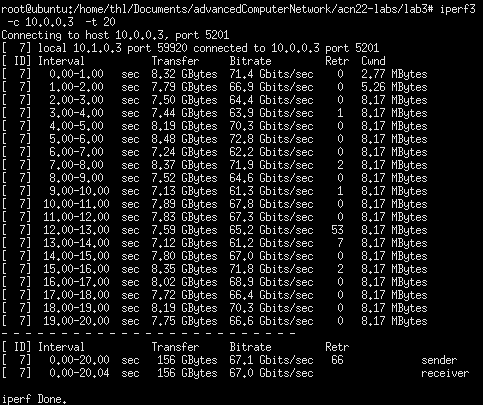
\includegraphics[width=7.5cm]{h003-h103-ft.png}
    \caption{Send packets from 10.1.0.3 to 10.0.0.3 with the two-level routing}
    \label{fig:e2ft}
    \end{minipage}
    \end{figure}
\end{itemize}




\end{document}
